% Explanation of how docker-based implementation of MedChain is developed + its components + how one can run and use this implementation.
% Also, will provide some figures to show an example of the docker-based network to illustrate what are the various components and how they are attached and interact with each other. 

In order to facilitate the deployment of (multi-node) MedChain network, docker-based deployment of it is enabled that uses docker images built for both MedChain server node and MedChain CLI client.
% An example of a network of 3 Medchain nodes with MedChain-cli-client is shown in Figure ??.

Docker-based deployment of MedChain is located in \texttt{deployment} directory of MedChain repository. Below, is the description of files found in this directory:

\begin{itemize}
    \item \texttt{Dockerfile}: Contains the commands needed to assemble MedChain node docker image
    \item \texttt{client.Dockerfile}: Dockerfile to build MedChain-cli-client docker image
    \item \texttt{docker-compose.yaml}: Multi-container definition of MedChain node and MedChain CLI client
    \item \texttt{docker-entrypoint.sh}: Docker entrypoint script for both MedChain node and MedChain CLI client containers
    \item \texttt{docker-compose-demo.yaml}: Multi-container definition of a network of 3 MedChain nodes and 1 MedChain CLI client (shown in Figure \ref{fig:demo-network}) which is also used in the demo.
\end{itemize}

\begin{figure}[htbp] 
        \centering 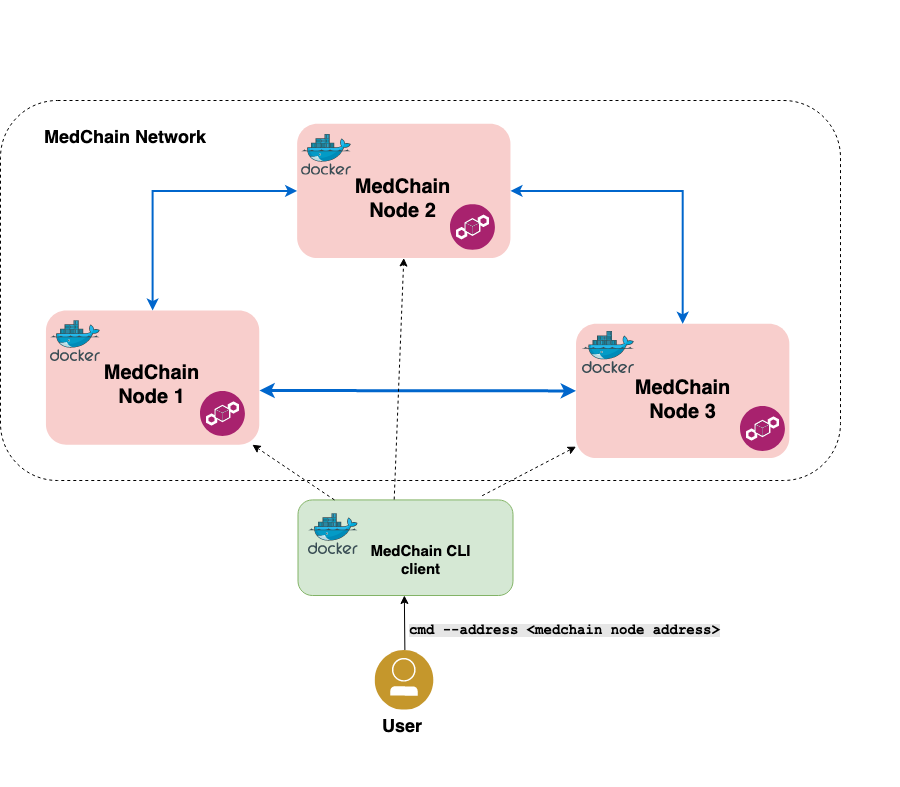
\includegraphics[width=1\columnwidth]{Images/demo.png}
        \caption{\label{fig:demo-network} 
         An example of a multi-node MedChain network created using the docker-based deployment of MedChain. This network is defined in \texttt{docker-compose-demo.yaml} file in \texttt{deployment} directory of MedChain. The user is able to interact with any of the three MedChain nodes (each running as a separate docker container) through \texttt{MedChain CLI Client} docker container by providing the address of MedChain node he/she wants to communicate with.   
        }
\end{figure}

\subsection{Use Docker to Run MedChain}

Docker can be used to run a MedChain node and its CLI client or a network of multiple MedChain nodes and CLI clients. 

To setup and run a single MedChain node and a single MedChain CLI client, and/or to build their docker images, one can run the following commands in \texttt{deployment/} directory of MedChain repository:

\begin{verbatim}
   bash$ docker-compose -f docker-compose.yaml up --build 
\end{verbatim}

This command will build MedChain server and CLI client images, setup and run the server in a container, and create a MedChain CLI client container that can interact with running server. Please note that flag \texttt{--build} is only necessary if the user needs to build docker images for MedChain node and its CLI client. 

Please note that before we can setup and run MedChain nodes using \texttt{docker-compose.yaml} file, we need to have the \texttt{private.toml} file of every MedChain node in \texttt{deployment/medchain-config/mcX} directory where X corresponds to node index. We can use the script \texttt{run\_nodes.sh} provided in \texttt{medchain-server} folder to setup as many MedChain nodes as we want. For example, to setup 3  MedChain nodes, we can use the command below:

\begin{verbatim}
    bash$ mkdir medchain-config
    bash$ ../cmd/medchain-server/run_nodes.sh -v 5 -n 3 -d ./medchain-config/
\end{verbatim}

Once all the servers are up and running, we need to use MedChain CLI client and run the commands in the running container, to this end, we can run:

\begin{verbatim}
   bash$ docker exec -it <name_of_cli_client_container> bash
\end{verbatim}

We can, then, use the commands described in Section \ref{section5} to interact with MedChain node through the CLI.  

To setup and run a multi-node network, one can define their own network in a docker-compose file and run it using:

\begin{verbatim}
   bash$ docker-compose -f <docker-compose file path> up  
\end{verbatim}


\textbf{Important point}: Once the network is up and running, we need to update the \texttt{private.toml} file of each node as well as \texttt{group.toml} file with the IP address of corresponding docker containers. To get the IP address of each container, we can use:

\begin{verbatim}
  bash$ docker network inspect <name of MedChain network>
\end{verbatim}
